В четвертой лабораторной работе мы займемся разработкой базовых классов самой игры, основываясь на готовой библиотеке, и определим классы отрисовки.


\subsection{Структура файлов проекта}
	
	Первая часть данной работы будет посвящена корректированию файловой структуры реализуемого проекта. Здесь мы выделим отдельно классы, отвечающие за библиотеки, и классы, отвечающие за реализацию игровой логики.

	Основной особенностью корректной файловой структуры в проекте является то, что она упрощает поиск файлов и доступ к ним. Возможность быстрого поиска файлов позволяет разработчикам быстрее выполнять поставленные перед ними задачи. 

	Также корректная структура файлов проекта может повысить согласованность кода и упростить совместное использование при разработке.

	Стандартная файловая структура проекта выглядит следующим образом:
	\begin{itemize}
		\item \inlinecoden{src/} (\textit{source}) -- папка, содержащая основные исходные файлы проекта. Здесь находятся файлы, используемые в разработке и сборке проекта;
		\item \inlinecoden{build/} -- папка, содержащая собранные файлы, используемые для дальнейшей публикации проекта;
		\item \inlinecoden{lib/} (\textit{library}) -- папка, содержащая в себе некоторый список файлов, библиотек, программ, скриптов или функций, которые затем используются в разработке;
		\item \inlinecoden{bin/} (\textit{binaries}) -- папка, содержая в себе исполняемые файлы проекта. Обычно добавляется в системные пути \inlinecode{PATH} (установка в систему);
		\item \inlinecoden{test/} -- папка, содержащая в себе все возможные тесты проекта, проводимые так же при сборке;
		\item \inlinecoden{config/} -- папка, содержащая в себе стандартные или пользовательские конфигурационные файлы;
		\item \inlinecoden{assets/} -- папка, содержащая в себе некоторый статический контект, представляющий из себя изображения, видео, аудио или шрифты.
	\end{itemize}

	Данный проект может содержать следующую структуру файлов (примерная, в зависимости от студента может отличаться):
	\begin{itemize}
		\item \inlinecoden{src/}
		\begin{itemize}
			\item \inlinecoden{src/Game/}
		\end{itemize}

		\item \inlinecode{lib/}
		\begin{itemize}
			\item \inlinecoden{lib/Math/}
			\begin{itemize}
				\item \inlinecoden{lib/Math/LowLevelMath}
				\item \inlinecoden{lib/Math/HighLevelMath}
			\end{itemize}
			\item \inlinecoden{lib/Engine/}
			\begin{itemize}
				\item \inlinecoden{lib/Engine/BasicClasses}
				\item \inlinecoden{lib/Engine/Visualization}
			\end{itemize}
			\item \inlinecoden{lib/Exceptions/}
			\begin{itemize}
				\item \inlinecoden{lib/Exceptions/MathExceptions}
				\item \inlinecoden{lib/Exceptions/EngineExceptions}
			\end{itemize}
		\end{itemize}

		\item \inlinecode{test/}
		\begin{itemize}
			\item \inlinecoden{test/UnitTests/}
			\begin{itemize}
				\item \inlinecoden{test/UnitTests/MathTests}
				\item \inlinecoden{test/UnitTests/EngineTests}
				\item \inlinecoden{test/UnitTests/GameTests}
			\end{itemize}
		\end{itemize}

		\item \inlinecode{config/}

	\end{itemize}


\subsection{Пересечение луча и плоскости}
	
	Рассмотрим пересечение луча и плоскости в $n$-мерном пространстве для нашего движка. Запишем известные данные:
	\begin{itemize}
		\item \( \un = \bracs{A_1, A_2, \cdots, A_n} \) -- вектор нормали к гиперплоскости;
		\item \( \ux^0 = \bracs{x_1^0, x_2^0, \cdots, x_n^0} \) -- вектор, описывающий начальную точку гиперплоскости;
		\item \( \ur = \bracs{\Delta x_1, \Delta x_2, \cdots, \Delta x_n} \) -- направляющий вектор прямой соответствующего луча;
		\item \( \ux^1 = \bracs{x_1^1, x_2^1, \cdots, x_n^1} \) -- вектор, описывающий начальную точку луча.
	\end{itemize}

	Уравнение пересечение гиперплоскости с прямой в $n$-мерном пространстве можно задать следующей системой уравнений:
	\[ \begin{cases} 
		A_1 \pares{x_1 - x_1^0} + A_2 \pares{x_2 - x_2^0} + \cdots + A_n \pares{x_n - x_n^0} = 0, \\
		\dfrac{x_1 - x_1^1}{\Delta x_1} = \dfrac{x_2 - x_2^1}{\Delta x_2} = \cdots = \dfrac{x_n - x_n^1}{\Delta x_n}.
	\end{cases} \]

	Вводя в уравнение прямой параметр $t \ge 0$, уравнение прямой можно записать в векторном виде:
	\[ \ux = \ux_1 + \ur \cdot t, ~ t \ge 0. \]
	Подставляя данную параметрическую систему уравнений в уравнение плоскости вместо соответствующих $x_k$, получим следующее уравнение:
	\[ \sum_{k = 1}^{n} A_k \cdot \pares{x_k^1 + \Delta x_k \cdot t - x_k^0} = 0, \]
	что можно записать в следующем виде:
	\[ \pares{\un, \ur \cdot t + \ux^1 - \ux^0} = 0. \]
	Раскрывая данное скалярное произведение, возможны следующие случаи:
	\begin{enumerate}
		\item В уравнении возможно выразить $t$. В таком случае, значение $t$, при котором уравнения плоскости и прямой имеют общую точку, можно выразить следующим образом:
			\[ \hat{t} = -\frac{ \pares{\un, \ux^1 - \ux^0} }{ \pares{\un, \ur} }. \]
			Подставляя найденное значение $t$ в параметрическое уравнение прямой, получим точку пересечения:
			\[ \ux = \ux_1 + \ur \cdot \hat{t}. \]
			В случае, если $t < 0$, луч не пересекает плоскость, так как сам задается только при неотрицательных $t$.

		\item В уравнении полностью сокращается $t$. Это возможно при условии, что \( \pares{\un, \ur} = 0 \). В таком случае возможны варианты, что луч или лежит в плоскости, или не пересекает ее. 

			Если \( \pares{\un, \ux^1 - \ux^0} = 0 \), то система уравнений пересечения прямой и плоскости выполняется, а значит луч лежит в плоскости для всех $t$. Расстояние между началом луча и точкой пересечения с плоскость равно нулю.
			
			В случае, если это равенство не выполняется, то, соответственно, не выполняется и система уравнений пересечения, а значит луч плоскость не пересекает, и является параллельным ей.
	\end{enumerate}


\subsection{Отправка лучей}
	
	Рассмотрим двумерный экран, описываемый прямоугольной областью размерности \( n \times m \) единиц (будем полагать за данные единицы количество разбиений на блоки по ширине и высоте экрана соответственно). Данный экран представляет собой некоторое отображение трехмерного мира на двумерную плоскость. Также будем рассматривать направляющий вектор $v$ и два угла \( \alpha, \beta \), описывающих горизонтальный и вертикальный углы обзора соответственно. Блоком с индексами \( i, j \) назовем блок на сетке \( n \times m \), отклоненный от направляющего вектора на угол \( \alpha_i, \beta_j \). В дополнение, переобозначим базисные вектора \( b_1, b_2, b_3 \) за вектора осей системы координат \( x, y, z \).

	Алгоритм заключается в построении матрицы всех возможных лучей, направляющихся в заданные блоки согласно заданным углам обзора и направляющему вектору. Полагаем, что направляющий вектор делит все возможные углы обзора пополам. Соответственно, при рассчете углов необходимо так же учитывать смещение \( \dfrac{\alpha}{2} \) и \( \dfrac{\beta}{2} \).

	Распишем алгоритм поэтапно:
	\begin{enumerate}
		\item Введем матрицу \( A: n \times m \), которая будет описывать все возможные лучи, отправляемые на экран;
		\item Построим изменения (дельты) углов согласно размерам экрана:
		\[ \Delta\alpha = \frac{\alpha}{n}, ~ \Delta\beta = \frac{\beta}{m}; \]
		\item Для каждой части экрана определим свое значение вертикального и горизонтального угла относительно направляющего вектора:
		\[ \alpha_i = \Delta \alpha \cdot i - \frac{\alpha}{2}, ~ \beta_j = \Delta \beta \cdot j - \frac{\beta}{2}, \quad i = \overline{0, n - 1}, ~ j = \overline{0, m - 1}. \]
		Таким образом мы получим, что:
		\[ \alpha_i \in \bracks{-\frac{\alpha}{2}, \frac{\alpha}{2}}, ~ \beta_j \in \bracks{-\frac{\beta}{2}, \frac{\beta}{2}}; \]
		\item Как только были получены углы, необходимо построить вектор \( v_{ij} \) путем поворота вектора $v$ в пространстве. Горизонтальный поворот будет осуществляться в плоскости \( XY \) (вокруг оси \( z \)) на угол \( \alpha_i \), а вертикальный в плокости \( XZ \) (вокруг оси \( y \)) на угол \( \beta_j \). Здесь ось $x$ считается направляющей; 
		\item Полученный вектор \( v_{ij} \) будет являться направляющим вектором для луча в блок с индексами \( i, j \). Таким образом, записываем луч с направляющим вектором \( v_{ij} \) в матрицу $A$ по индексам \( i, j \).
	\end{enumerate}

	В результате преобразования проецируемой плоскостью станет сектор сферы, так как в преобразовании поворота вектора не изменяли размер: \( \abs{v_{ij}} = \abs{v} \).

	Рассмотрим случай, в котором перед зрителем стоит плоскость, параллельная плоскости экрана, и необходимо получить проекцию этой плоскости на экран. В случае рассмотренного алгоритма возникнет ситуация, в которой чем дальше блок от центра экрана (направляющего вектора), тем дальше будет проекция в блоке. Это можно проиллюстрировать на следующем изображении:

	\begin{figure}[H]
		\centering
		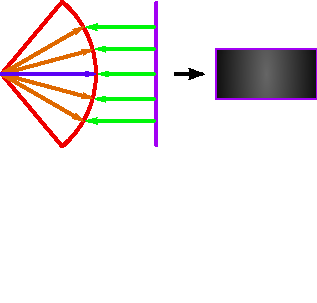
\includegraphics[width=0.5\textwidth]{additional/fisheye1.pdf}
		\caption{Демонстрация эффекта}
	\end{figure}

	Такой эффект носит название эффекта <<рыбьего глаза>>. Для исправления такого эффекта необходимо, чтобы длина проекции на направляющий вектор каждого отклоненного вектора c некоторым коэффициентом масштабирования \( \tilde{v}_{ij} = k v_{ij} \) совпадала с длиной самого направляющего вектора:
	\[ \abs{\Pr\pares{\tilde{v}_{ij}, v}} \equiv \abs{v}. \]
	Таким образом необходимо найти такое значение $k$, при котором это условие выполняется.

	Положим, что угол между векторами $v$ и \( v_{ij} \) в пространстве равен \( \gamma \). Тогда:
	\[ \abs{\Pr\pares{v_{ij}, v}} = \abs{v} \cos{\gamma}, \]
	при этом
	\( \abs{\tilde{v}_{ij}} = \abs{k} \cdot \abs{v_{ij}} \), и по свойству оператора проецирования \( \abs{\Pr\pares{\tilde{v}_{ij}, v}} = \abs{\Pr\pares{k \cdot v_{ij}, v}} = \abs{k} \cdot \abs{\Pr\pares{v_{ij}, v}} \). Разделяя на \( \cos{\gamma} \), получим коэффициент масштабирования:
	\[ k = \sec{\gamma} \implies \tilde{v}_{ij} = v_{ij} \cdot \sec{\gamma}. \]
	Угол между двумя векторами можно получить из формулы скалярного произведения двух векторов:
	\[ \pares{v, v_{ij}} = \abs{v} \cdot \abs{v_{ij}} \cdot \cos{\gamma} \implies \sec{\gamma} = \frac{\abs{v} \cdot \abs{v_{ij}}}{\pares{v, v_{ij}}} = \frac{\abs{v}^2}{\pares{v, v_{ij}}}. \]

	Таким образом,
	\[ \tilde{v}_{ij} = v_{ij} \sec{\gamma} = \frac{\abs{v}^2}{\pares{v, v_{ij}}} \cdot v_{ij}. \]

	Полученный результат можно проиллюстрировать на следующем изображении:
	\begin{figure}[H]
		\centering
		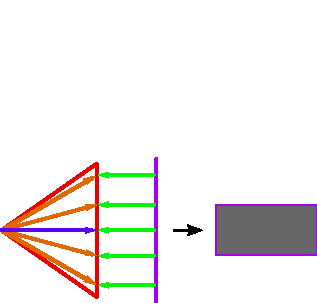
\includegraphics[width=0.5\textwidth]{additional/fisheye2.pdf}
		\caption{Метод исправления полученного эффекта}
	\end{figure}

	Здесь может возникнуть ситуация, когда \( \pares{v, v_{ij}} = 0 \). Она может возникнуть в том случае, если вектора ортогональны друг другу, что может возникнуть при условии, что углы обзора содержат в себе значения, не меньшие $\pi$. Соответственно, такой угол не является допустимым в рамках данной реализации. 


\subsection{Класс Ray}
	\noindent Реализуемые методы:
	\begin{enumerate}
		\item \inlinecode{normalize()} -- метод, выполняющий нормировку направляющего вектора в луче.
	\end{enumerate}


\subsection{Класс Game.Object}
	\noindent Реализуемые методы:
	\begin{enumerate}
		\item \inlinecode{intersection_distance(ray: Ray) -> float} -- метод поиска расстояния от начала луча до точки пересечения луча с объектом. В глобальном классе считается пустым методом, возвращающим по умолчанию \inlinecode{0}. Для каждого объекта задается индивидуально.
	\end{enumerate}


\subsection{Класс Game.Camera[\textit{Game.Object}]}
	Для камеры необходимо прописать метод рассчета лучей, полученных путем алгоритма, описанного выше:

	\noindent Реализуемые методы:
	\begin{enumerate}
		\item \inlinecode{get_rays_matrix(n, m: int) -> Matrix\{n, m\}[[Ray]]} -- метод, с помощью которого получаются все возможные лучи.
	\end{enumerate}

	Данный метод может работать корректно только в случае, когда камера является камерой с направляющим обзор вектором (\inlinecode{direction}). В случае, если камера задается точкой обзора (\inlinecode{look_at}), необходимо обработать такой случай отдельно, и вычислить нормированный направляющий вектор по двум точкам -- позиция камеры и точка обзора.


\subsection{Класс Game.HyperPlane[\textit{Game.Object}]}
	Здесь необходимо перейти к модулю, описывающему уже конкретную игру, и создать в нем объект плоскости.

	\noindent Инициализация:
	\begin{enumerate}
		\item \inlinecode{Game.HyperPlane(position: Point, normal: Vector)} -- класс гиперплоскости, заданной в некотором положении в заданной системе координат с вектором нормали к гиперплоскости. При инициализации вызывается метод \inlinecode{set_property} для заданных аргументов. Вектор направления необходимо нормировать в заданном векторном пространстве.
	\end{enumerate}

	\noindent Перегружаемые методы:
	\begin{enumerate}
		\item \inlinecode{planar_rotate(inds: (int, int), angle: float) -> None} -- повернуть нормаль гиперплоскости в пространстве.
		\item \inlinecode{rotate_3d(angles: (float, float, float)) -> None} -- повернуть трехмерную плоскость на заданные углы;
		\item \inlinecode{intersection_distance(ray: Ray) -> float} -- метод нахождения расстояния от начала луча до точки пересечения плоскости и луча.
	\end{enumerate}


\subsection{Класс Game.HyperEllipsoid[\textit{Game.Object}]}

	\noindent Инициализация:
	\begin{enumerate}
		\item \inlinecode{Game.HyperEllipsoid(position: Point, direction: Vector, semiaxes: list[float])} -- класс гиперэллипса, заданного в некотором положении в заданной системе координат, повернутый по заданному вектору направления, с соответствующими $n$-полуосями.
	\end{enumerate}

	\noindent Перегружаемые методы:
	\begin{enumerate}
		\item \inlinecode{planar_rotate(inds: (int, int), angle: float) -> None} -- повернуть гиперэллипс в пространстве.
		\item \inlinecode{rotate_3d(angles: (float, float, float)) -> None} -- повернуть трехмерный эллипсоид на заданные углы;
		\item \inlinecode{intersection_distance(ray: Ray) -> float} -- метод нахождения расстояния от начала луча до точки пересечения гиперэллипса и луча.
	\end{enumerate}


\subsection{Класс Game.Canvas}

	Данный класс описывает базовый <<холст>> для отрисовки. Уже содержит в себе всю информацию об игре (список сущностей, систему координат).

	\noindent Инициализация:
	\begin{enumerate}
		\item \inlinecode{Game.Canvas(n, m: int)} -- размер экрана.
	\end{enumerate}

	\noindent Реализуемые поля:
	\begin{enumerate}
		\item \inlinecode{n(int), m(int)} -- размерность экрана;
		\item \inlinecode{distances(Matrix\{n, m\}[[float]])} -- матрица расстояний. Необходима для отрисовки.
	\end{enumerate}

	\noindent Реализуемые методы:
	\begin{enumerate}
		\item \inlinecode{draw() -> None} -- метод, производящий отрисовку в классе \inlinecode{Game} известной матрицы \inlinecode{distances};
		\item \inlinecode{update(camera: Game.Camera) -> None} -- метод, обновляющий матрицу \inlinecode{distances} согласно виду из камеры. Производит полный пробег по всем сущностям \inlinecode{EntityList}, на основе которых с помощью метода \inlinecode{intersection_distance} строит новую матрицу \inlinecode{distances}.
	\end{enumerate}


\subsection{Этапы реализации}

	Зафиксируем представленные классы в поэтапной реализации движка:
	\begin{enumerate}
		\item Сформируем логическую структуру файлов в проекте;
		\item Реализуем рассчет и отправку лучей из камеры с учетом разрешения эффекта <<рыбьего глаза>>;
		\item Введем несколько дополнительных методов для класса луча и игрового объекта;
		\item Внутри игры создадим два наследуемых игровых объекта -- гиперплоскость и гиперэллипс, для которых пропишем методы пересечения с лучем;
		\item Создадим класс полотна, которое в дальнейшем будем использовать для отрисовки объектов;
		\item Провести тестирование для отрисовки лучей и пересечения лучей с объектами -- гиперплоскостями и гиперэллипсами, а также проверить корректность рассчета дистанций до объекта с исправлением эффекта <<рыбьего глаза>>.
	\end{enumerate}

